\pend
\newpage [p.~15]
\begin{center}
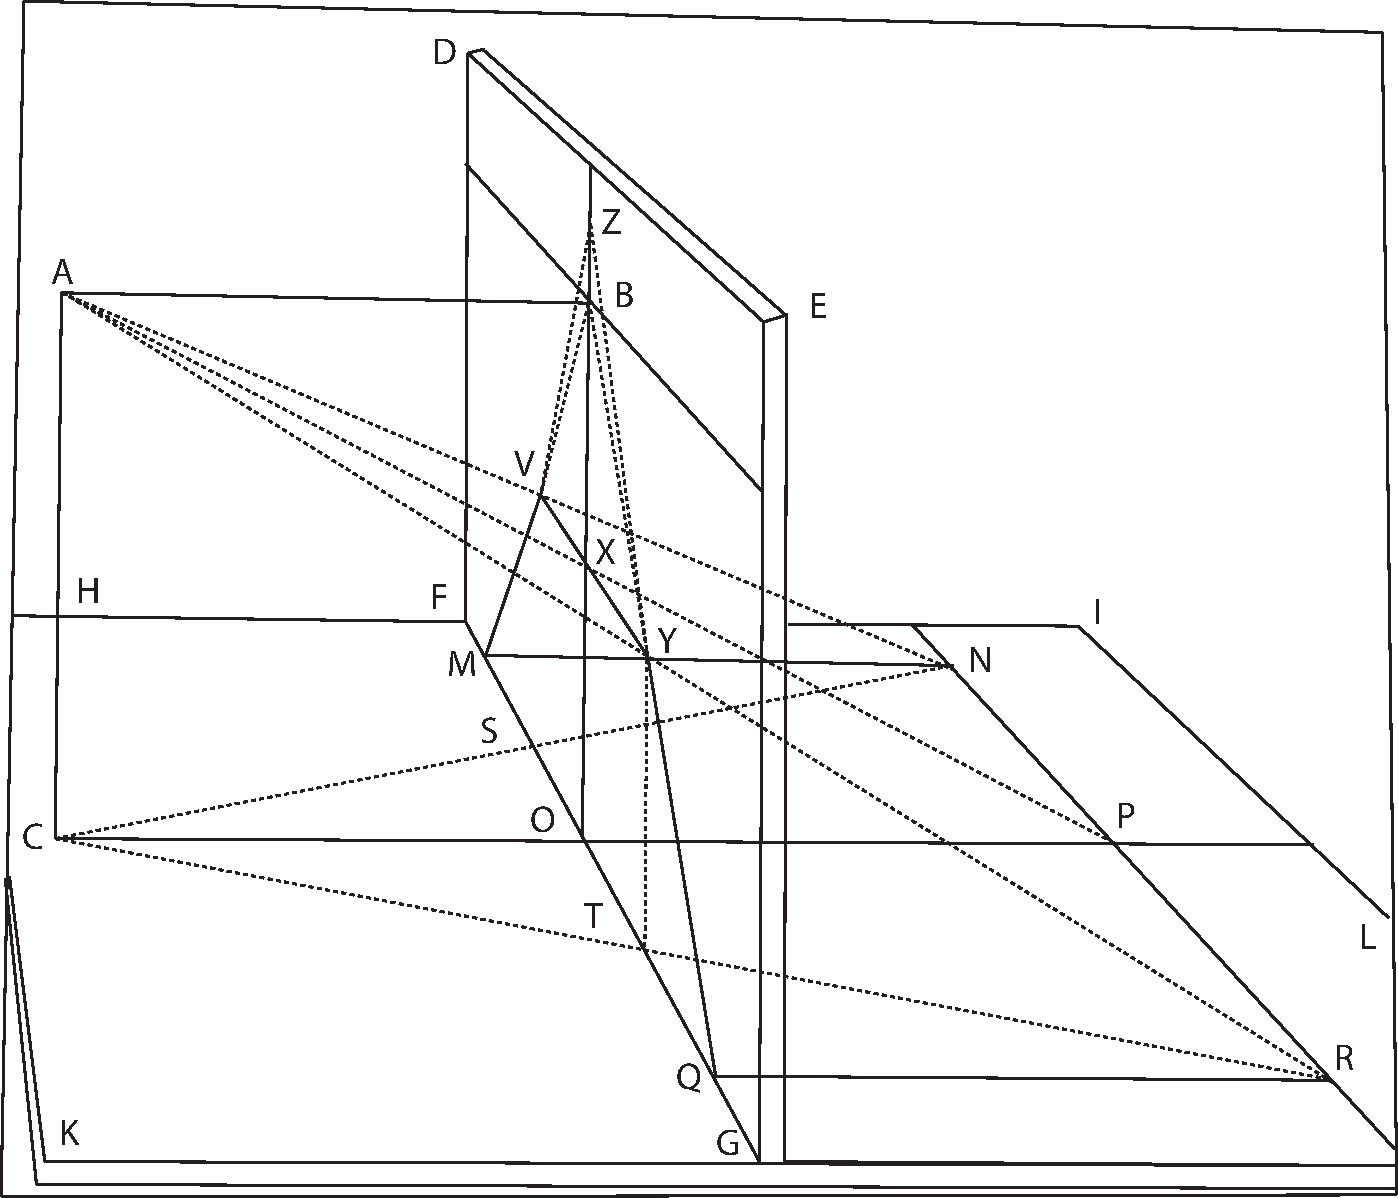
\includegraphics[width=1\textwidth]{images/Aleaume_15}
\\\rule[-4mm]{0mm}{10mm}\textit{[Fig. 1]}\footnote{\textit{Neben der Zeichnung rechts:} ob $\bigtriangledown$\textsuperscript{la} \textit{CST, CNR} similia \\
\protect\begin{tabular}{rcl}$CP$&&$CN.\hspace{5.5pt}CR.\hspace{5.5pt} NR$\\&ergo&\\dupl.\hspace{5.5pt}$CP$&&dupl.$\hspace{5.5pt} CS.\hspace{5.5pt} CT.\hspace{5.5pt} SO$ \protect\end{tabular} 
ob $\bigtriangledown$\textsuperscript{la}\textit{ACR, YTR} similia} 
\end{center}
\pstart
                 